\documentclass{article}

\usepackage{graphicx}
\usepackage{tikz}
\usepackage{tikzsymbols}
\usetikzlibrary{calc,patterns,shapes.geometric}
\pagestyle{empty}
\usepackage[margin=0pt]{geometry}
\geometry{papersize={14in,12in}}

\def\centerarc[#1](#2)(#3:#4:#5){\draw[#1] ($(#2)+({#5*cos(#3)},{#5*sin(#3)})$) arc (#3:#4:#5);}

\begin{document}
	\begin{figure}
		\centering
		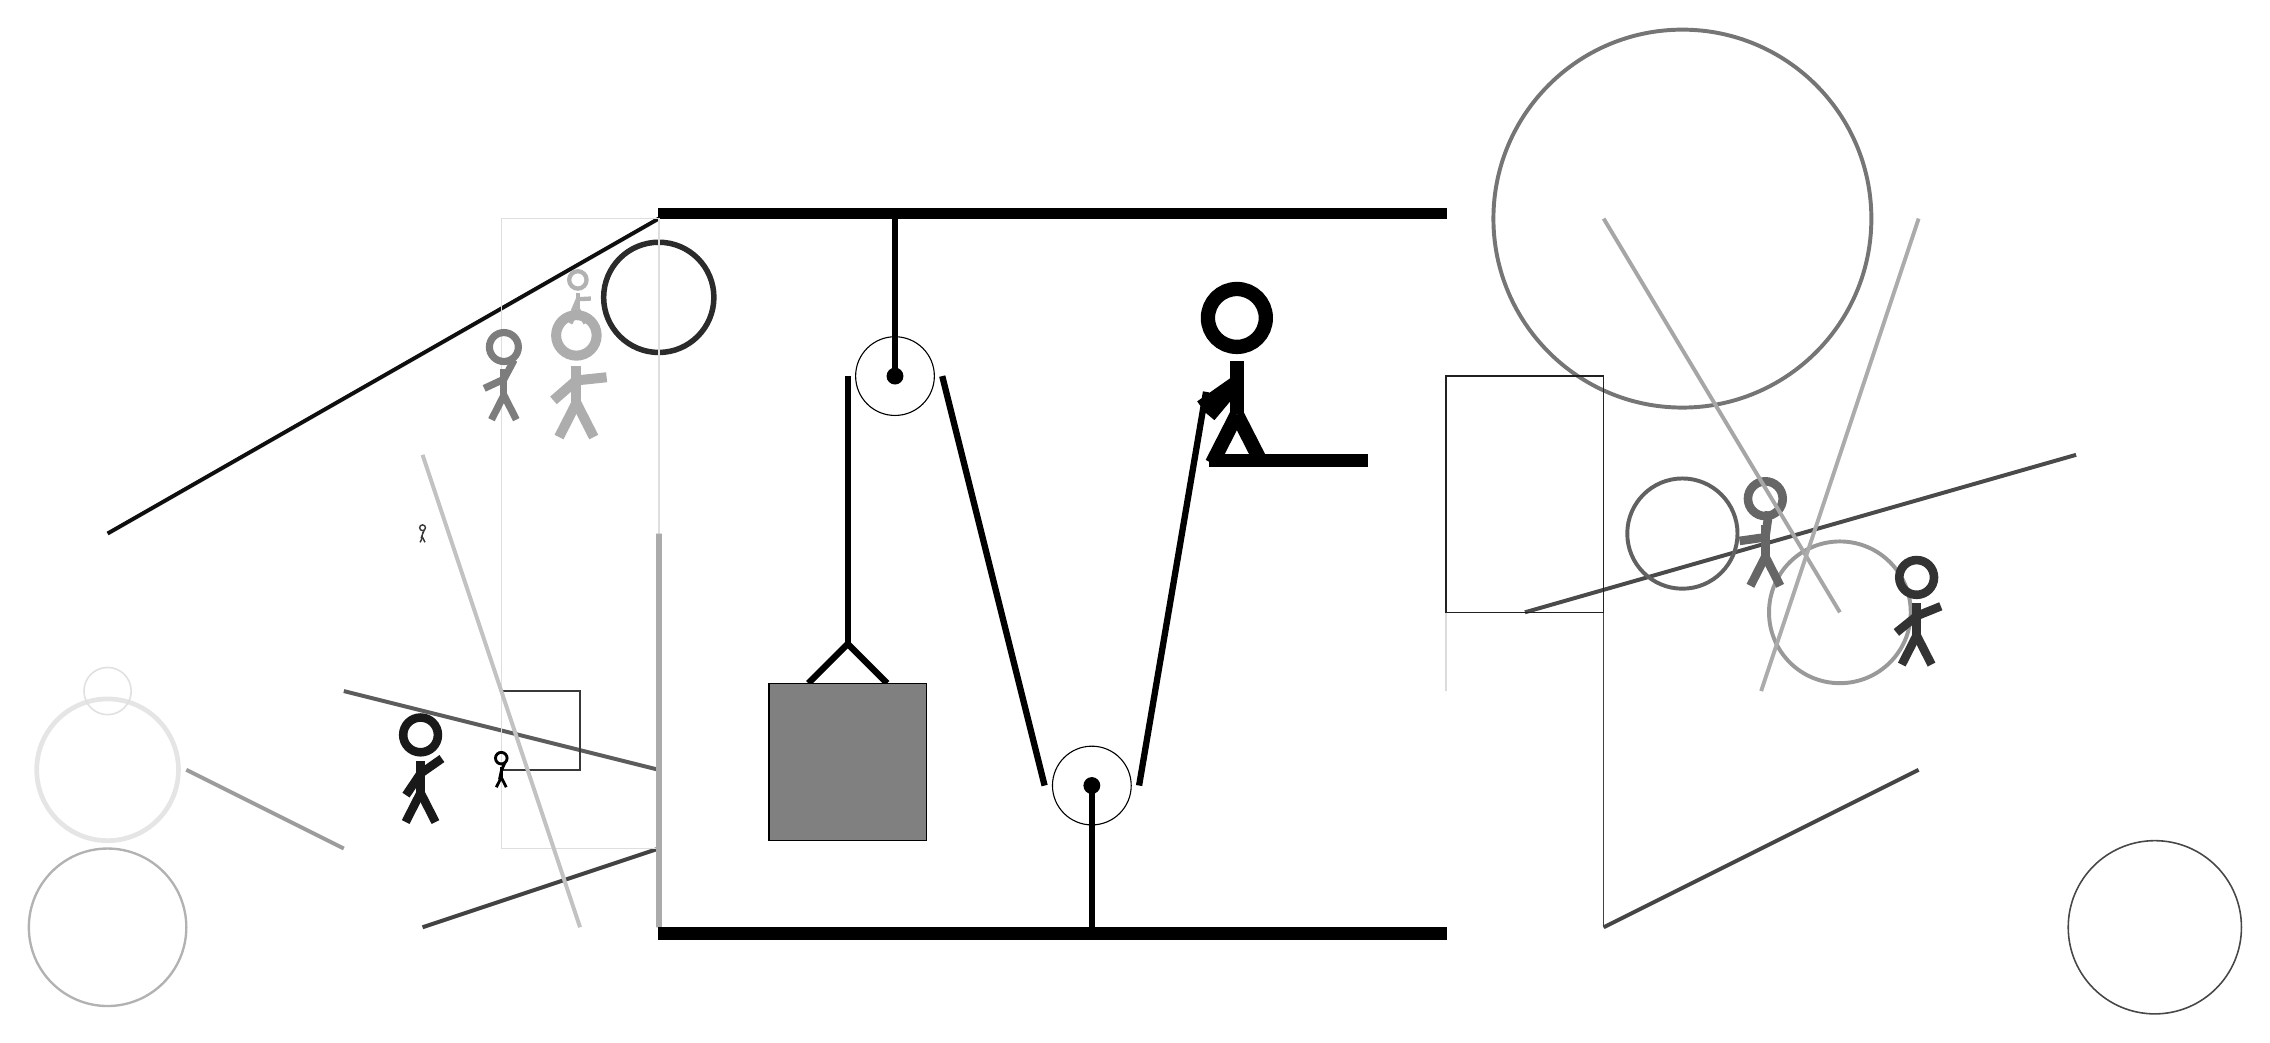
\begin{tikzpicture}
			%%%%% START %%%%%
			
			\draw[fill=black] (-2, 9) rectangle (8, 9.125);
			
			\draw (3.5, 1.8) circle (0.5);
			\draw[fill=black] (3.5, 1.8) circle (0.1);
			\draw[line width=0.8mm] (3.5, 1.8) -- (3.5, 0);
			
			\draw (1, 7) circle (0.5);
			\draw[fill=black] (1, 7) circle (0.1);
			\draw[line width=0.8mm] (1, 9) -- (1, 7);
			
			\draw[line width=0.8mm](-0.1, 3.1) --  (0.4, 3.6) -- (0.9, 3.1);
			\draw[fill=black!50] (-0.6, 3.1) rectangle (1.4, 1.1);
			
			\draw[line width=0.8mm](0.4, 7) -- (0.4, 3.6);
			\centerarc[line width=0.8mm](1, 7)(180:0:0.6)
			\draw[line width=0.8mm](1.6, 7) -- (2.9, 1.8);
			\centerarc[line width=0.8mm](3.5, 1.8)(180:360:0.6)
			\draw[line width=0.8mm](4.1, 1.8) -- (4.95, 6.8);
			
			\node at (5.3, 7) {\Strichmaxerl[10][35][-130]};
			\draw[fill=black] (5, 6) rectangle (7, 5.85);
			
			\draw[line width=0.5mm, color=black!64](-6, 3) -- (-2, 2);
			
			\draw [line width=0.7mm, color=black!83](-2, 8) circle (0.7);
			\draw[line width=0.5mm, color=black!71](9, 4) -- (16, 6);
			\draw [line width=0.5mm, color=black!62](11, 5) circle (0.7);
			\draw[line width=0.2mm, color=black!78] (-4, 3) rectangle (-3, 2);
			
			\draw[line width=0.2mm, color=black!74] (10, 6) rectangle (10, 0);
			\draw[line width=0.5mm, color=black!74](-2, 1) -- (-5, 0);
			\node[line width=0.7mm, color=black!90] at (-5, 2) {\Strichmaxerl[6][56][35]};
			\draw[line width=0.5mm, color=black!94](-2, 9) -- (-9, 5);
			\draw [line width=0.5mm, color=black!54](11, 9) circle (2.4);
			\draw [line width=0.5mm, color=black!40](13, 4) circle (0.9);
			\node[line width=0.5mm, color=black!78] at (-5, 5) {\Strichmaxerl[1][70][67]};
			\draw [line width=0.6mm, color=black!10](-9, 2) circle (0.9);
			
			\draw[line width=0.2mm, color=black!14] (8, 5) rectangle (8, 3);
			\node[line width=0.3mm, color=black!60] at (12, 5) {\Strichmaxerl[6][8][82]};
			\draw[line width=0.5mm, color=black!73](10, 0) -- (14, 2);
			
			\draw[line width=0.2mm, color=black!13] (-4, 9) rectangle (-2, 1);
			\node[line width=0.5mm, color=black!100] at (-4, 2) {\Strichmaxerl[2][78][67]};
			\draw[line width=0.2mm, color=black!87] (8, 7) rectangle (10, 4);
			
			\draw [line width=0.2mm, color=black!72](17, 0) circle (1.1);
			\draw [line width=0.2mm, color=black!12](-9, 3) circle (0.3);
			
			\node[line width=0.7mm, color=black!30] at (-3, 8) {\Strichmaxerl[3][67][3]};
			\draw[line width=0.7mm, color=black!33] (-2, 0) rectangle (-2, 5);
			\draw[line width=0.5mm, color=black!24](-3, 0) -- (-5, 6);
			\draw [line width=0.3mm, color=black!30](-9, 0) circle (1.0);
			
			\node[line width=0.3mm, color=black!51] at (-4, 7) {\Strichmaxerl[5][25][62]};
			\draw [line width=0.6mm, color=black!15](-5, 4) circle (0.0);
			\draw[line width=0.5mm, color=black!35](13, 4) -- (10, 9);
			
			\node[line width=0.4mm, color=black!80] at (14, 4) {\Strichmaxerl[6][39][22]};
			\draw[line width=0.5mm, color=black!39](-6, 1) -- (-8, 2);
			\node[line width=0.5mm, color=black!32] at (-3, 7) {\Strichmaxerl[7][41][6]};
			\draw[line width=0.5mm, color=black!33](12, 3) -- (14, 9);
			
			\draw[fill=black] (-2, 0) rectangle (8, -0.15);
			
			%%%%% END %%%%%
		\end{tikzpicture}
	\end{figure}	
\end{document}